% Created 2014-11-04 星期二 12:48
\documentclass[table]{beamer}
\usepackage{fixltx2e}
\usepackage{graphicx}
\usepackage{longtable}
\usepackage{float}
\usepackage{wrapfig}
\usepackage{soul}
\usepackage{textcomp}
\usepackage{marvosym}
\usepackage{wasysym}
\usepackage{latexsym}
\usepackage{amssymb}
\usepackage{hyperref}
\tolerance=1000
\usepackage{etex}
\usepackage{amsmath}
\usepackage{pstricks}
\usepackage{pgfplots}
\usepackage{tikz}
\usepackage[europeanresistors,americaninductors]{circuitikz}
\usepackage{colortbl}
\usepackage{yfonts}
\usetikzlibrary{shapes,arrows}
\usetikzlibrary{positioning}
\usetikzlibrary{arrows,shapes}
\usetikzlibrary{intersections}
\usetikzlibrary{calc,patterns,decorations.pathmorphing,decorations.markings}
\usepackage[BoldFont,SlantFont,CJKchecksingle]{xeCJK}
\setCJKmainfont[BoldFont=Evermore Hei]{Evermore Kai}
\setCJKmonofont{Evermore Kai}
\usepackage{pst-node}
\usepackage{pst-plot}
\psset{unit=5mm}
\mode<beamer>{\usetheme{Frankfurt}}
\mode<beamer>{\usecolortheme{dove}}
\mode<article>{\hypersetup{colorlinks=true,pdfborder={0 0 0}}}
\mode<beamer>{\AtBeginSection[]{\begin{frame}<beamer>\frametitle{Topic}\tableofcontents[currentsection]\end{frame}}}
\setbeamercovered{transparent}
\subtitle{频率特性分析}
\providecommand{\alert}[1]{\textbf{#1}}

\title{线性系统的频域分析法}
\author{}
\date{}
\hypersetup{
  pdfkeywords={},
  pdfsubject={},
  pdfcreator={Emacs Org-mode version 7.9.3f}}

\begin{document}

\maketitle

\begin{frame}
\frametitle{Outline}
\setcounter{tocdepth}{3}
\tableofcontents
\end{frame}













\section{频域性能分析}
\label{sec-1}
\begin{frame}
\frametitle{稳定裕度}
\label{sec-1-1}

\begin{itemize}
\item 相角裕度 $\gamma$ : $\gamma=180^{\circ}+\phi(\omega_c)$
\item 幅值裕度 $h$ : $h=-20\lg A(\omega_x)$
\end{itemize}
\end{frame}
\begin{frame}
\frametitle{Nyquist 图与稳定裕度}
\label{sec-1-2}

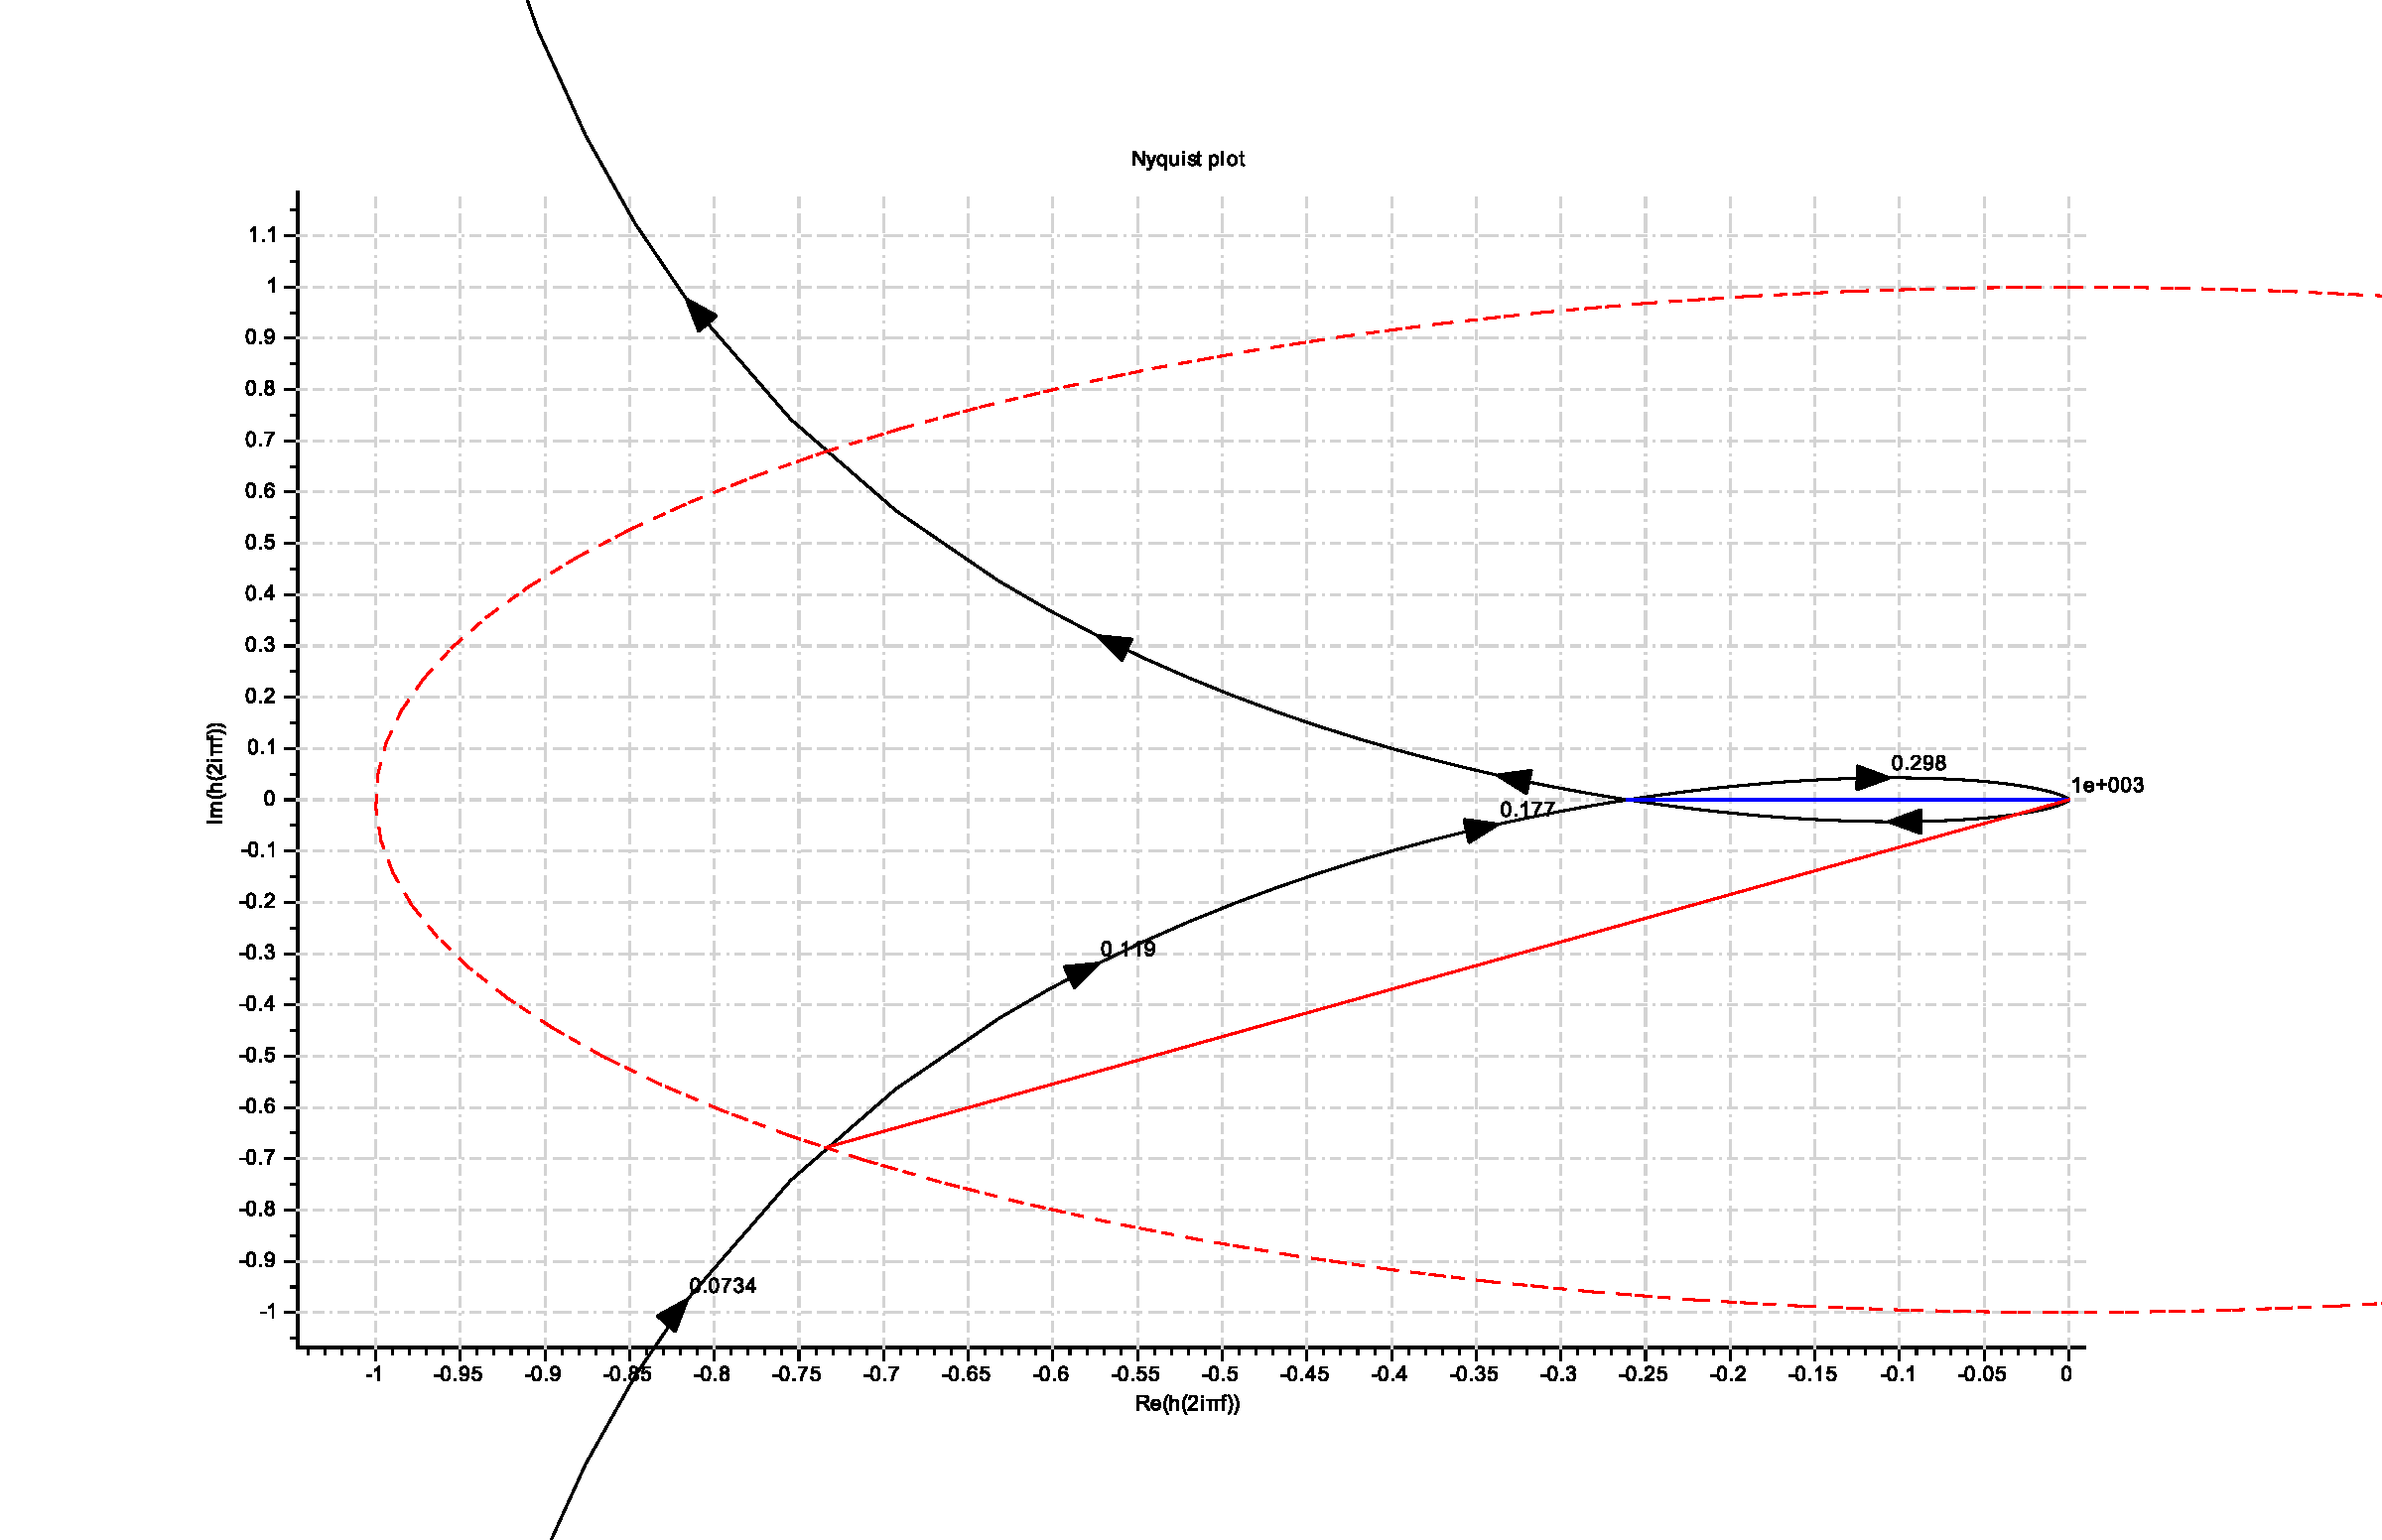
\includegraphics[width=.9\linewidth]{image/margin_nyquist_scilab.pdf}
\end{frame}
\begin{frame}
\frametitle{Bode 图与稳定裕度}
\label{sec-1-3}

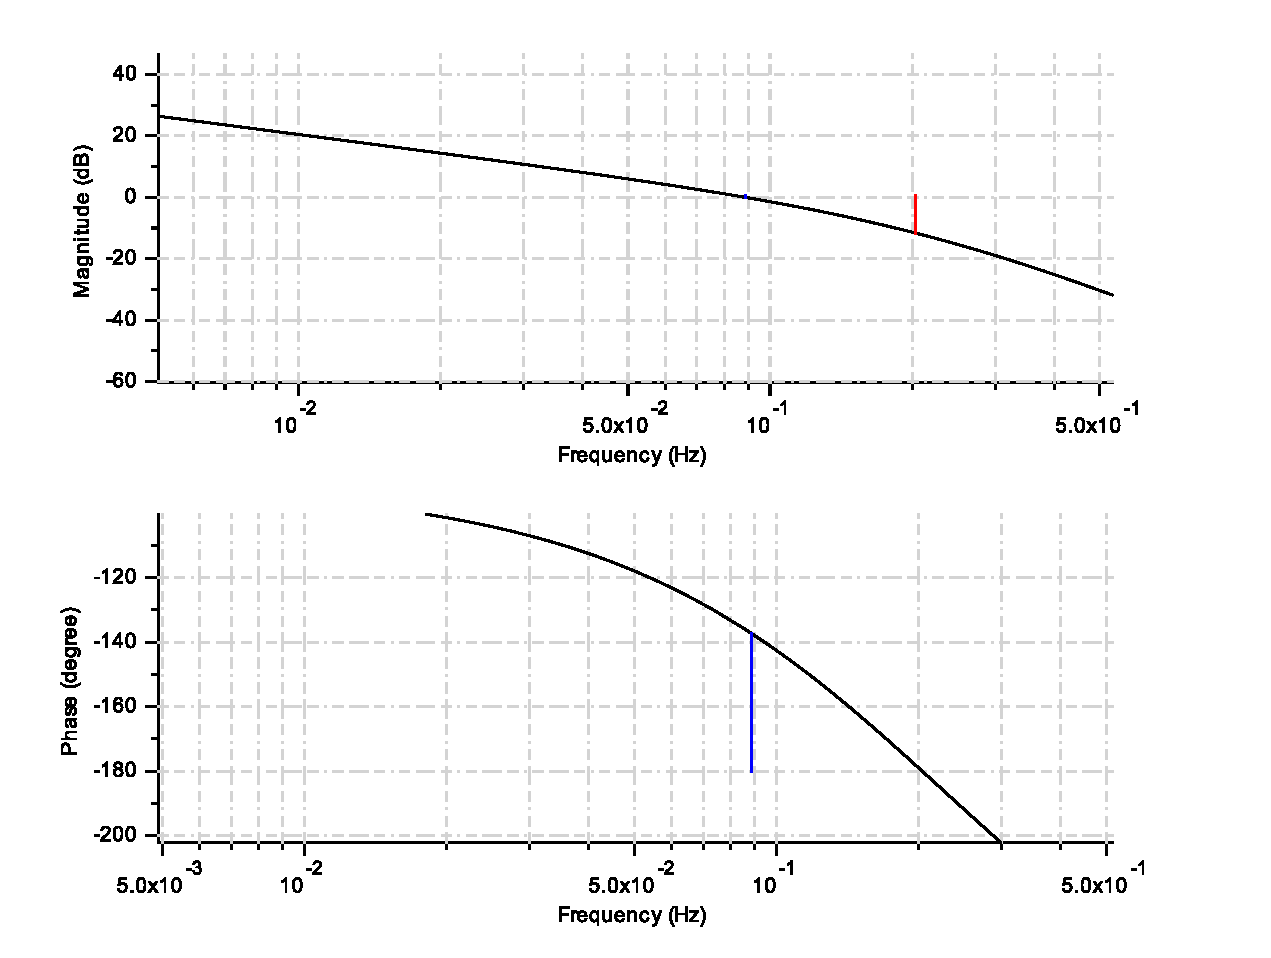
\includegraphics[width=.9\linewidth]{image/margin_bode_scilab.pdf}
\end{frame}
\begin{frame}
\frametitle{$\omega_c$ 近似计算}
\label{sec-1-4}

 例: $G_o(s)=\frac{100(s+4)}{s(s+1)(s+2)(s+3)}$ 近似计算求解 $\omega_c$ 
\begin{itemize}
\item <3->$\omega_c<1$   时, $A(\omega)=\frac{200}{3}\cdot\frac{1}{\omega_c}$ , $\omega_c=\frac{200}{3}>2$ 矛盾.
\item <4->$1<\omega_c<2$ 时, $A(\omega)=\frac{200}{3}\cdot\frac{1}{\omega_c\cdot\omega_c}$ , $\omega_c=\sqrt{\frac{200}{3}}>2$ 矛盾.
\item <5->$2<\omega_c<3$ 时, $A(\omega)=\frac{200}{3}\cdot\frac{1}{\omega_c\cdot\omega_c\cdots\frac{\omega_c}{2}}$ , $\omega_c=\sqrt[3]{\frac{400}{3}}>3$ 矛盾.
\item <6->$2<\omega_c<3$ 时, $A(\omega)=\frac{200}{3}\cdot\frac{1}{\omega_c\cdot\omega_c\cdots\frac{\omega_c}{2}\cdots\frac{\omega_c}{3}}$ , $\omega_c=\sqrt[4]{400}>4$ 矛盾.
\item <7->$2<\omega_c<3$ 时, $A(\omega)=\frac{200}{3}\cdot\frac{\frac{\omega_c}{4}}{\omega_c\cdot\omega_c\cdots\frac{\omega_c}{2}\cdots\frac{\omega_c}{3}}$ , $\omega_c=\sqrt[3]{100}>4$ 成立.
\end{itemize}
\end{frame}
\begin{frame}
\frametitle{频带宽度}
\label{sec-1-5}

\begin{itemize}
\item 设闭环系统频率特性为 $\Phi(j\omega)$ , 若 $\omega>\omega_b$ 时,有 $20\lg|\Phi(j\omega)| <20\lg|\Phi(j0)|-3$ ,则称 $\omega_b$ 为带宽频率.

      \begin{tikzpicture}
      \draw[->] (-1,0) -- (4.5,0);
      \draw[->] (0,-0.5) -- (0,2);
      %\draw[dashed] (-4,-5) -- (-4,0);
      \draw [red] plot [smooth] coordinates {(0,1) (1,1)  (2,1.2) (2.5,0.70795) (3,0.2) };
      \draw (0,1) node[left] {$1$};
      \draw (0,0) node[below left] {$o$};
      \draw[pink,dashed] (2,0)-- ++(0,1.2);
      \draw (2,0) node[below] {$\omega_r$};
      \draw[pink,dashed] (0,1.2)--++(2,0);
      \draw (0,1.2) node[above left] {$M_r$};
      \draw[blue,dashed] (2.5,0)-- ++(0,0.70795);
      \draw (2.5,0) node[below] {$\omega_b$};
      \draw[blue,dashed] (0,0.70795)--++(2.5,0);
      \end{tikzpicture}
\end{itemize}
\end{frame}
\section{闭环频率特性的确定}
\label{sec-2}
\begin{frame}
\frametitle{等 $\alpha$ 曲线}
\label{sec-2-1}

\begin{align*}
G(j\omega) &= Ae^{j\phi} \\
\Phi(j\omega) &= Me^{j\alpha}\\
 &= \frac{Ae^{j\phi}}{1+Ae^{j\phi}}\\
\frac{Ae^{j\phi}}{Me^{j\alpha}}&=1+Ae^{j\phi} \\
\frac{A}{M}&=e^{-j(\phi-\alpha)}+Ae^{j\alpha}\\
0 &= \sin(\alpha-\phi)+A\sin\alpha\\
20\lg A &=20\lg\frac{\sin(\phi-\alpha)}{\sin\alpha}
\end{align*}
\end{frame}
\begin{frame}
\frametitle{等 $M$ 曲线}
\label{sec-2-2}

\begin{align*}
\frac{Ae^{j\phi}}{Me^{j\alpha}}&=1+Ae^{j\phi} \\
\frac{A}{M}&=|1+Ae^{j\phi}|\\
\frac{A^2}{M^2}&=(1+A\cos\phi)^2+A^2\sin^2\phi\\
0 &=(1-M^{-2})A^2+2\cos\phi A+1\\
A &= \frac{\cos\phi\pm\sqrt{\cos^2\phi+M^{-2}-1}}{M^{-2}-1}\\
20\lg A &=20\lg \frac{\cos\phi\pm\sqrt{\cos^2\phi+M^{-2}-1}}{M^{-2}-1}
\end{align*}
\end{frame}
\begin{frame}
\frametitle{Nichols Chart}
\label{sec-2-3}

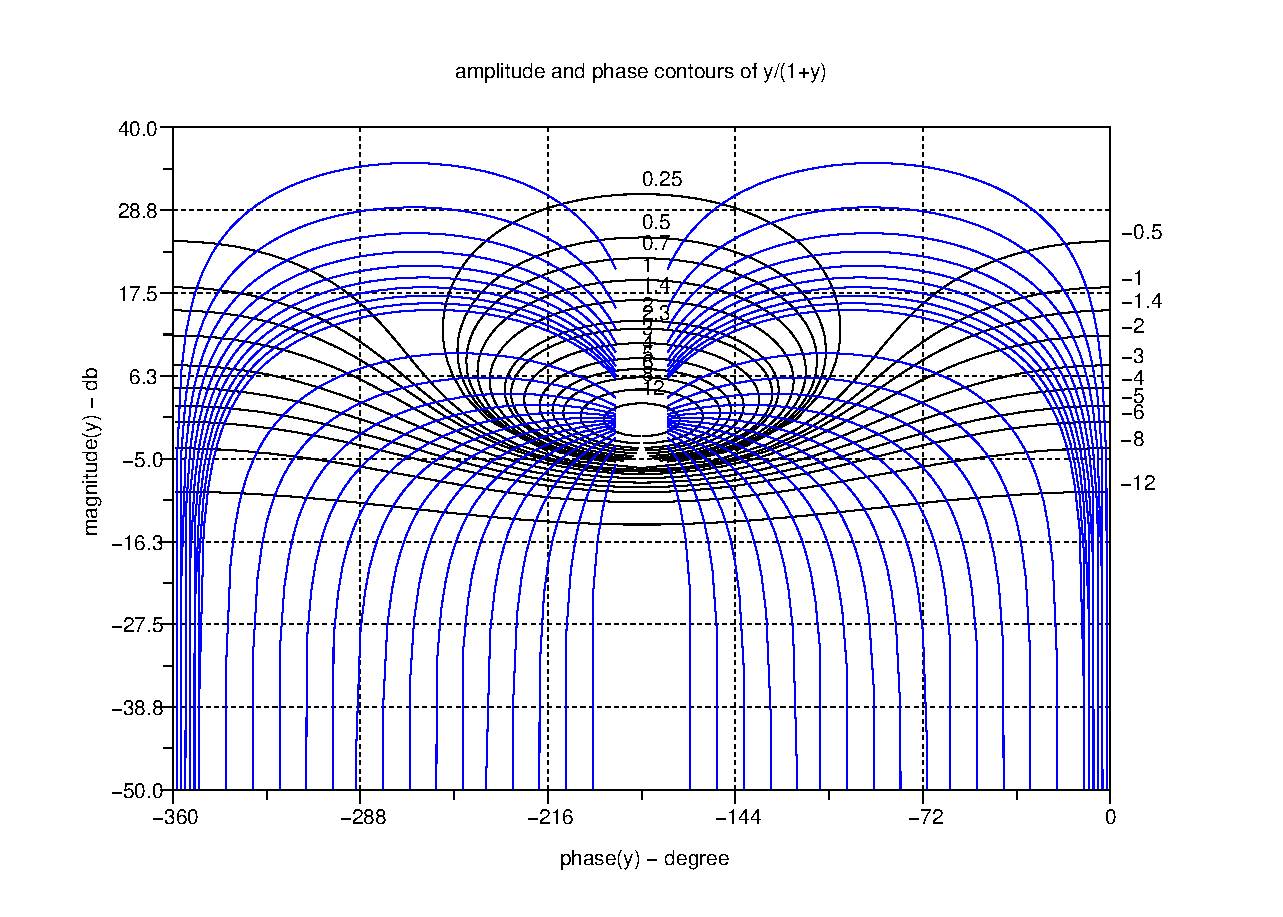
\includegraphics[width=.9\linewidth]{image/nichols_chart.eps}
\end{frame}
\section{指标转换}
\label{sec-3}
\begin{frame}
\frametitle{系统闭环和开环和频域指标的关系}
\label{sec-3-1}

\begin{align*}
G(j\omega) &= Ae^{-j(180^{\circ}-\gamma(\omega))}\\
&=A\left( -\cos\gamma(\omega)-j\sin\gamma(\omega)\right)\\
M&=\left|\frac{G(j\omega)}{1+G(j\omega)}\right| \\
 &=\frac{A}{\sqrt{1+A^2-2A\cos\gamma(\omega)}}\\
 &=\frac{1}{\sqrt{\left[\frac{1}{A}-\cos\gamma(\omega)\right]^2+\sin^2\gamma(\omega)}}\\
M_r &= \frac{1}{\sin\gamma(\omega_r)} \approx \frac{1}{sin\gamma}\qquad (\omega_r \approx \omega_c)
\end{align*}
\end{frame}
\begin{frame}
\frametitle{2阶系统频域指标}
\label{sec-3-2}

\begin{align*}
G(j\omega) &= \frac{\omega_n^2}{j\omega(j\omega+2\xi\omega_n)}\\
&=\frac{\omega_n^2}{\omega\sqrt{\omega^2+4\xi^2\omega_n^2}}\angle(-\arctan \frac{\omega}{2\xi\omega_n}-90^{\circ})\\
\omega_c &=\omega_n(\sqrt{4\xi^4+1}-2\xi^2)^{\frac{1}{2}}\\
\gamma &= 180^{\circ}+\angle G(j\omega_c) \\
 &=\arctan \frac{2\xi\omega_n}{\omega_c}
\end{align*}
\end{frame}
\begin{frame}
\frametitle{2阶系统频域指标( $M_r,\omega_r$ )}
\label{sec-3-3}

\begin{eqnarray*}
M_r & = &\frac{1}{2\xi\sqrt{1-\xi^2}} \\
\omega_r &=& \omega_n\sqrt{1-2\xi^2}
\end{eqnarray*}
\begin{itemize}
\item <2->$M_r$ 与 $\sigma\%$ 一一对应,且成正比
\end{itemize}
\end{frame}
\begin{frame}
\frametitle{高阶系统频域指标}
\label{sec-3-4}
\begin{columns}
\begin{column}{0.7\textwidth}
%% 经验公式
\label{sec-3-4-1}

\begin{eqnarray*}
M_r & = & \frac{1}{\sin\gamma}\\
\sigma\% &=& 16\%+0.4(M_r-1), (1\leq M_r\leq 1.8) \\
t_s &=& \frac{K\pi}{\omega_c}\\
K&=& 2+1.5(M_r-1)+2.5(M_r-1)^2 
\end{eqnarray*}

\begin{itemize}
\item <2->$\gamma\uparrow \rightarrow \sigma\%\downarrow \rightarrow \xi\uparrow$  一一对应
\item <3->$\omega_c\uparrow \rightarrow t_s\downarrow$ (快速性)
\end{itemize}
\end{column}
\begin{column}{0.3\textwidth}
\begin{block}<4->{频域要求:}
\label{sec-3-4-2}

\begin{itemize}
\item 低频段:稳态性能
\item 中频段:瞬态性能
\item 高频段:抗干扰能力
\end{itemize}
\end{block}
\end{column}
\end{columns}
\end{frame}

\end{document}
